\documentclass[12pt]{article}
\usepackage{mathtools}
\addtolength{\textheight}{.5in}
\addtolength{\textwidth}{1in}
\addtolength{\topmargin}{-.25in}
\addtolength{\evensidemargin}{-.5in}
\addtolength{\oddsidemargin}{-.5in}
\usepackage{placeins}
\begin{document}

\section{Relate $\Omega_{j}$ and $\omega_{j}$ in terms of $h$}
$$ \frac{\rho_{i} + \rho_{k} + \rho_{\Lambda}} {\rho_{c}} =  \frac{\rho_{i} + \rho{k} + \rho{\Lambda}}{\frac{3H^{2}}{8\pi G}} = \Omega_{i} + \Omega_{k} + \Omega_{\Lambda}$$
$$ \frac{\rho_{i} + \rho_{k} + \rho_{\Lambda}}{\frac{3(100 h)^{2}}{8\pi G}} = \Omega_{i} + \Omega_{k} + \Omega_{\Lambda} $$
$$ (\omega_{i} + \omega_{k} + \omega_{\Lambda})/h^{2} =  \Omega_{i} + \Omega_{k} + \Omega_{\Lambda} $$
$$ \omega_{i} + \omega_{k} + \omega_{\Lambda} = h^{2}( \Omega_{i} + \Omega_{k} + \Omega_{\Lambda}) $$

\section{Write the Friedmann Equation in terms of $\omega_{j}$ and $h$}
From the Friedmann equation we have
$$ \frac{8\pi G}{3}( \rho_{i} + \rho_{k} + \rho_{\Lambda}) = H^{2}$$
$$\rho_{i} + \rho_{k} + \rho_{\Lambda} = \frac{3H^{2}}{8\pi G}$$
Dividing both sides of the second expression by $\rho^{100}_{c}$ gives us
$$\omega_{i} + \omega_{k} + \omega_{\Lambda} = \rho_{c} / \rho^{100}_{c} = h^{2}$$

\section{Find the value of $\rho^{100}_{c}$ in energy units}
From the back of K\&T The critical density is quoted as $8.0992h^{2} \times 10^{-47} \mathrm{GeV}^{4}$. To get $\rho^{100}_{c}$ we let h go to 1 here, to get
$\rho^{100}_{c} = 8.0992 \times 10^{-47} \mathrm{GeV}^{4}$

\section{Matlab code attached}

\section{Find $\omega_{r}$ using accounting for neutrinos}
K\&T gives the value of $8.09 \times 10^{-34} \mathrm{g} \, \mathrm{cm}^{-3}$ or $8.09 \times 10^{-31} \mathrm{Kg} \, \mathrm{m}^{-3}$. Now to convert this to energy units, multiply by $c$ and divide by  $(\hbar c)^{-3}$ to get $3.487 \times 10^{-15} \mathrm{eV}^{4}$ or $3.487 \times 10^{-51} \mathrm{GeV}^{4}$. This yields $\rho_{r} = 3.487 \times 10^{-51} \mathrm{GeV}^{4} \, a^{-4}$, and after dividing by  $\rho^{100}_{c}$ gives

$$ \omega_{r} = 4.305 \times 10^{-5} \, a^{-4} $$

\section{Find when matter and radiation densities are equal}
$$\rho_{m}(a_{eq}) = \rho_{r}(a_{eq})$$
$$ .958 \times 10^{-47} \, a_{eq}^{-3} =  3.487 \times 10^{-51}  \, a_{eq}^{-4}$$
$$ a_{eq} = 3.487 \times 10^{-51} / .958 \times 10^{-47} = 3.64 \times 10^{-4}$$

\section{Plots}
\FloatBarrier
included on the next pages
\begin{figure}
\centering
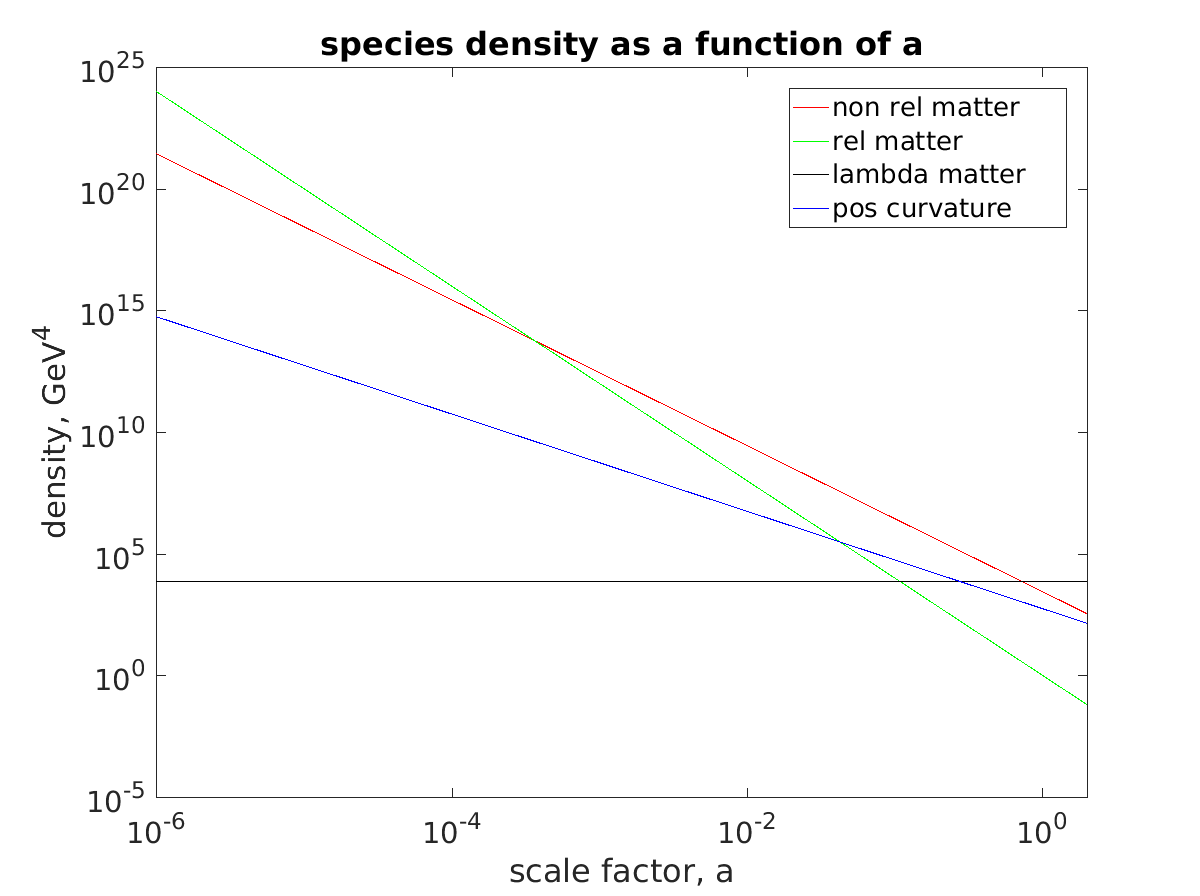
\includegraphics[width=6in]{rho_k_pos.png}
\caption{using a curvature density with positive initial condition}
\end{figure}

\begin{figure}
\centering
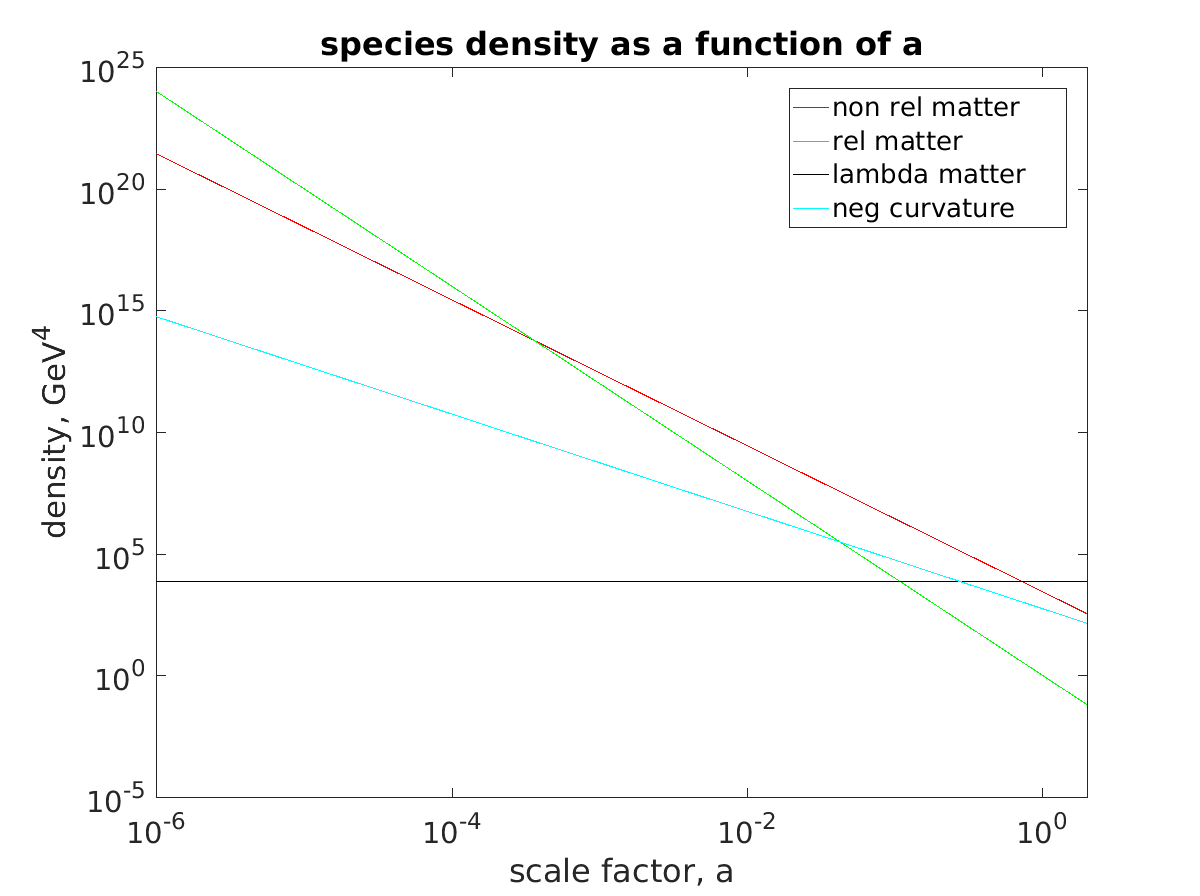
\includegraphics[width=6in]{rho_k_neg.png}
\caption{using a curvature density with negative initial condition}
\end{figure}

\begin{figure}
\centering
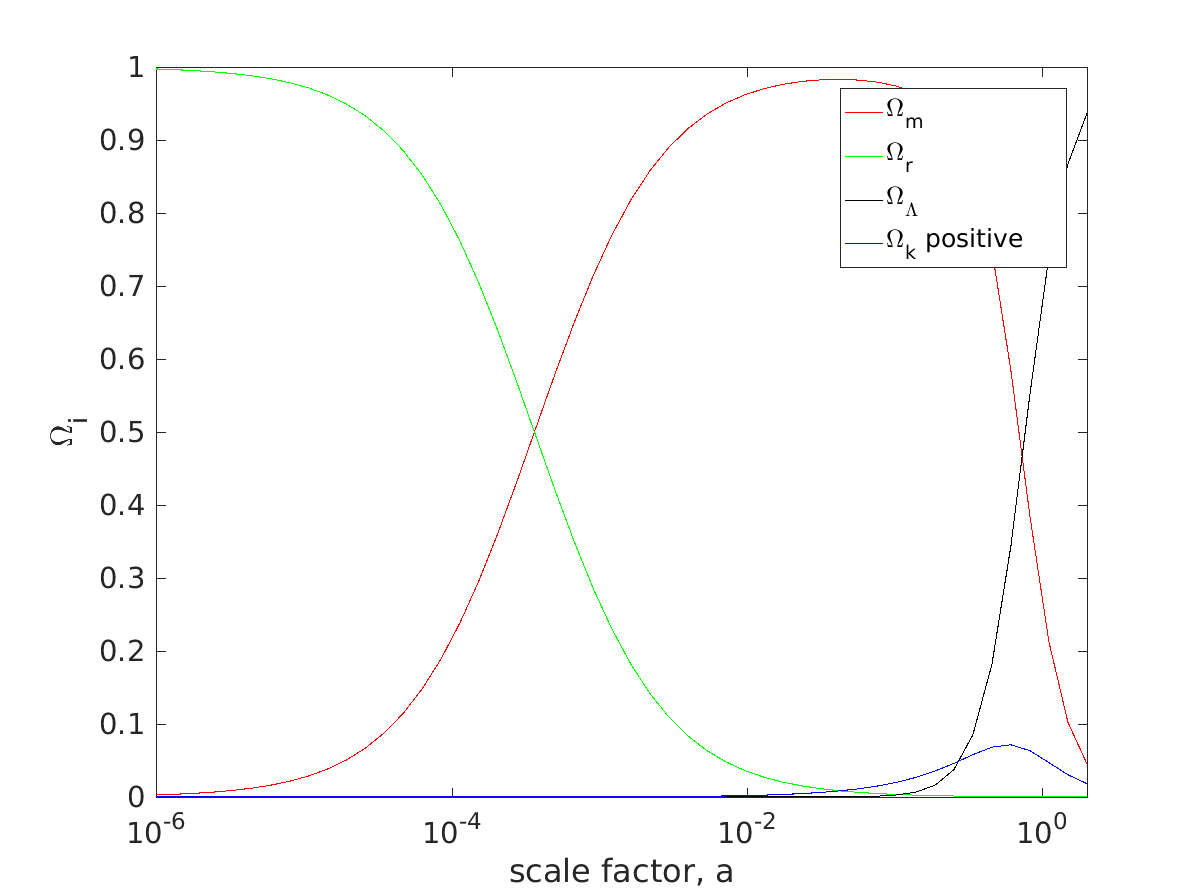
\includegraphics[width=6in]{Omega_k_pos.png}
\caption{using a curvature density with positive initial condition}
\end{figure}

\begin{figure}
\centering
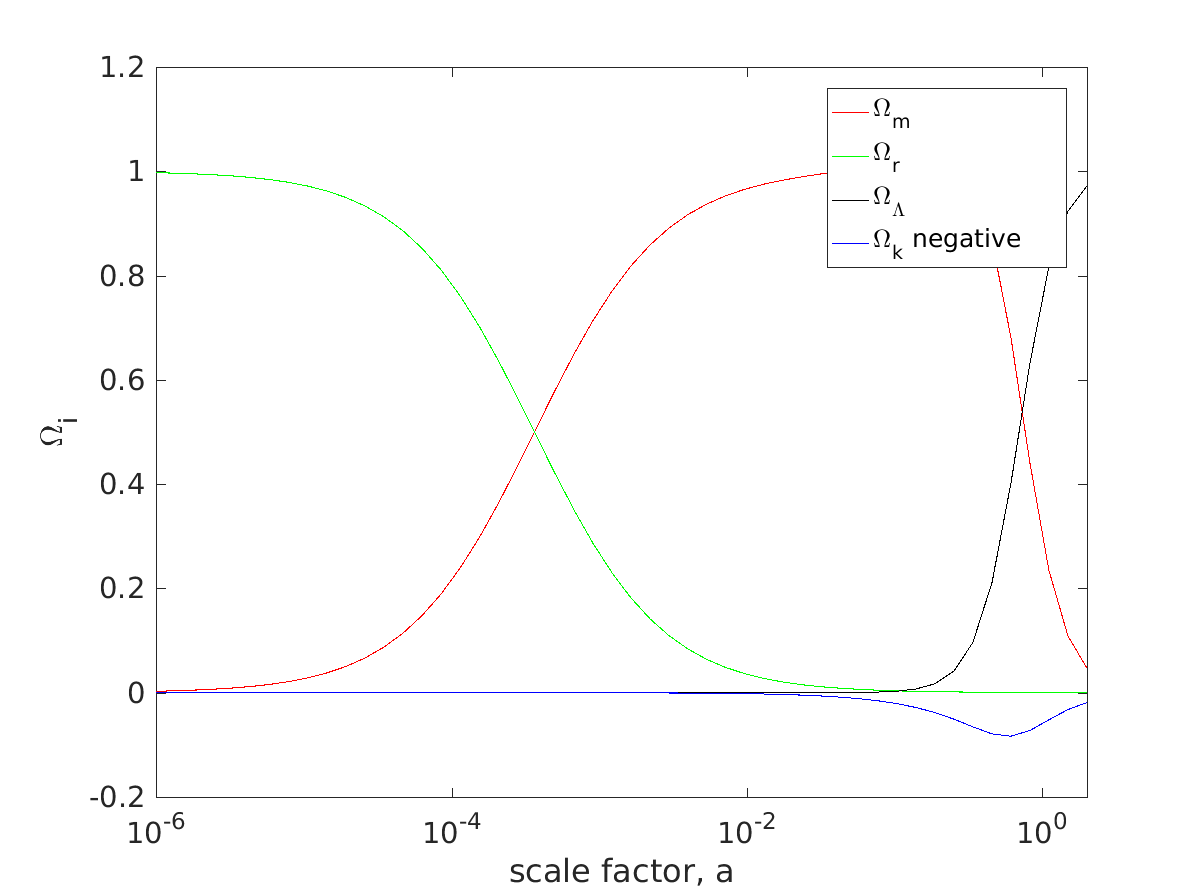
\includegraphics[width=6in]{Omega_k_neg.png}
\caption{using a curvature density with negative initial condition}
\end{figure}

\end{document}